\documentclass[12pt, notitlepage, final]{article} 

\newcommand{\name}{Vince Coghlan}

\usepackage{amsfonts}
\usepackage{amssymb}
\usepackage{amsmath}
\usepackage{latexsym}
\usepackage{enumerate}
\usepackage{amsthm}
\usepackage{nccmath}
\usepackage{setspace}
\usepackage[pdftex]{graphicx}
\usepackage{epstopdf}
\usepackage[siunitx]{circuitikz}
\usepackage{tikz}
\usepackage{float}
\usepackage{cancel} 
\usepackage{setspace}
\usepackage{overpic}
\usepackage{mathtools}
\usepackage{listings}
\usepackage{color}

\numberwithin{equation}{section}
\DeclareRobustCommand{\beginProtected}[1]{\begin{#1}}
\DeclareRobustCommand{\endProtected}[1]{\end{#1}}
\newcommand{\dbr}[1]{d_{\mbox{#1BR}}}
\newtheorem{lemma}{Lemma}
\newtheorem*{corollary}{Corollary}
\newtheorem{theorem}{Theorem}
\newtheorem{proposition}{Proposition}
\theoremstyle{definition}
\newtheorem{define}{Definition}
\newcommand{\column}[2]{
\left( \begin{array}{ccc}
#1 \\
#2
\end{array} \right)}

\newdimen\digitwidth
\settowidth\digitwidth{0}
\def~{\hspace{\digitwidth}}

\setlength{\parskip}{1pc}
\setlength{\parindent}{0pt}
\setlength{\topmargin}{-3pc}
\setlength{\textheight}{9.0in}
\setlength{\oddsidemargin}{0pc}
\setlength{\evensidemargin}{0pc}
\setlength{\textwidth}{6.5in}
\newcommand{\answer}[1]{\newpage\noindent\framebox{\vbox{{\bf ECEN 3000 Spring 2014} 
\hfill {\bf \name} \vspace{-1cm}
\begin{center}{Prelab \#2}\end{center} } }\bigskip }

%absolute value code
\DeclarePairedDelimiter\abs{\lvert}{\rvert}%
\DeclarePairedDelimiter\norm{\lVert}{\rVert}
\makeatletter
\let\oldabs\abs
\def\abs{\@ifstar{\oldabs}{\oldabs*}}
%
\let\oldnorm\norm
\def\norm{\@ifstar{\oldnorm}{\oldnorm*}}
\makeatother

\def\dbar{{\mathchar'26\mkern-12mu d}}
\def \Frac{\displaystyle\frac}
\def \Sum{\displaystyle\sum}
\def \Int{\displaystyle\int}
\def \Prod{\displaystyle\prod}
\def \P[x]{\Frac{\partial}{\partial x}}
\def \D[x]{\Frac{d}{dx}}
\newcommand{\PD}[2]{\frac{\partial#1}{\partial#2}}
\newcommand{\PF}[1]{\frac{\partial}{\partial#1}}
\newcommand{\DD}[2]{\frac{d#1}{d#2}}
\newcommand{\DF}[1]{\frac{d}{d#1}}
\newcommand{\fix}[2]{\left(#1\right)_#2}
\newcommand{\ket}[1]{|#1\rangle}
\newcommand{\bra}[1]{\langle#1|}
\newcommand{\braket}[2]{\langle #1 | #2 \rangle}
\newcommand{\bopk}[3]{\langle #1 | #2 | #3 \rangle}
\newcommand{\Choose}[2]{\displaystyle {#1 \choose #2}}
\newcommand{\proj}[1]{\ket{#1}\bra{#1}}
\def\del{\vec{\nabla}}
\newcommand{\avg}[1]{\langle#1\rangle}
\newcommand{\piecewise}[4]{\left\{\beginProtected{array}{rl}#1&:#2\\#3&:#4\endProtected{array}\right.}
\newcommand{\systeme}[2]{\left\{\beginProtected{array}{rl}#1\\#2\endProtected{array}\right.}
\def \KE{K\!E}
\def\Godel{G$\ddot{\mbox{o}}$del}

\onehalfspacing

\begin{document}

\answer{}

1) \textbf{5.6:}
\begin{figure}[H]
\begin{center}
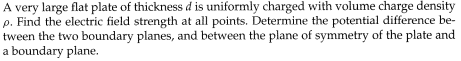
\includegraphics[width=14cm]{f1}
\end{center}
\end{figure}

Above and below the plate, the elecric feild from the plate is the integral:
\[
  \int_{-d/2}^{d/2} \frac{\rho}{2\epsilon_0} dy = \frac{\rho d}{2 \epsilon_0}
\]
Inside the plate, the field is the superposition of the fields from the top and
bottom of the plate.  The field from the above boundary plate is:
\[
  \frac{\rho(y-d/2)}{2\epsilon_0}
\]
And from below:
\[
  \frac{\rho(y+d/2)}{2\epsilon_0}
\]
Where $y$ is the distance from the center of the plate.  The sum of this is the
field that at the point $y$:
\[
  \frac{\rho y}{\epsilon_0}
\]
The potential difference between the boundary plates is:
\[
  \int_{-d/2}^{d/2} \frac{\rho y}{\epsilon_0} dy = \frac{\rho (d/2)^2}{2\epsilon_0} - \frac{\rho (-d/2)^2}{2\epsilon_0} = 0
\]
To move it out to the boundary plane we modify the bounds of the integral:
\[
  \int_{0}^{d/2} \frac{\rho y}{\epsilon_0} dy = \frac{\rho (d/2)^2}{2\epsilon_0} = \frac{\rho d^2}{8\epsilon_0}
\]

\newpage

2) \textbf{5.14:}
\begin{figure}[H]
\begin{center}
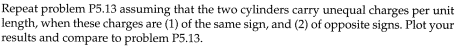
\includegraphics[width=14cm]{f2}
\end{center}
\end{figure}
First I will do problem 5.13, which asks me to find an expression for the electric field strength
and potential between and outside two long coaxial cylinders of radii $a$ and $b$ $(b>a)$, carrying
charges $Q'$ and $-Q'$ per unit length. (This structure is known as a coaxial cable, or coaxial line.)
Plot your resuls.  Determine the voltage between the two cylinders.  The electric field is going to
be the superposition of the fields from both wires.  For the inner wire:
\[
  \oint_S E \cdot dS = E(r) 2\pi rh = \frac{Q}{\epsilon_0} \Rightarrow E(r) = \frac{Q'}{2\pi \epsilon_0 r}
\]
The outer cylinder contributes the opposite field. This creates a net field of 0 outside of both
cylinders.  In between the cylinders, the field will only be the field contributed by the inner
wire, this is because of how Gauss' law allows us to make our integrating surface in the middle
of the wires and ignore the outside one.  The electric field is therefore:
\[
  \frac{Q'}{2\pi \epsilon_0 r}
\]
The plot if $a = 0.5$ and $b = 4$ looks like:
\begin{figure}[H]
\begin{center}
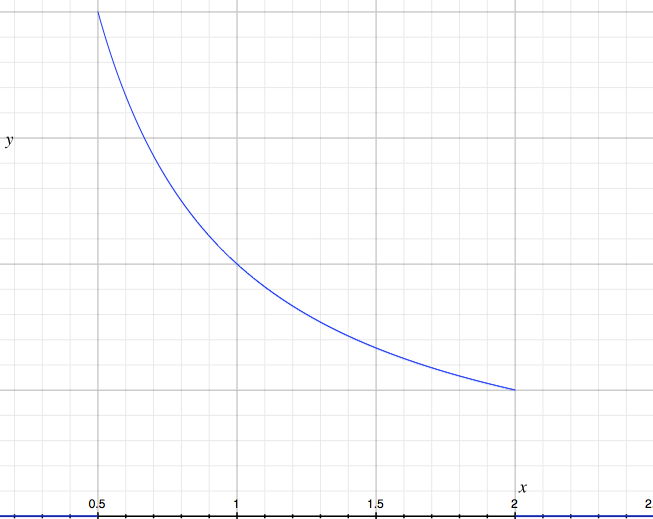
\includegraphics[width=10cm]{p1}
\end{center}
\end{figure}

This allows us to find the potential difference by integrating the electric field:
\[
  \int_{a}^{b} \frac{Q'}{2\pi \epsilon_0 r} dr = \frac{Q'}{2\pi \epsilon_0}\ln{\frac{b}{a}}
\]
Now we will look at unequal charges, first of the same sign.  These will be represented as $\lambda_a$
and $\lambda_b$.  In this case the electric field inside will be the electric field from the inner
wire, or $\frac{\lambda_a}{2\pi \epsilon_0 r}$.  Outside of both wires these fields will sum together
and look like the following:
\[
  \frac{\lambda_a + \lambda_b}{2\pi \epsilon_0 r}
\]
The potential is found in the same way:
\[
  \frac{\lambda_a + \lambda_b}{2\pi \epsilon_0}\ln\frac{b}{a}
\]
Our plot is going to change slightly:
\begin{figure}[H]
\begin{center}
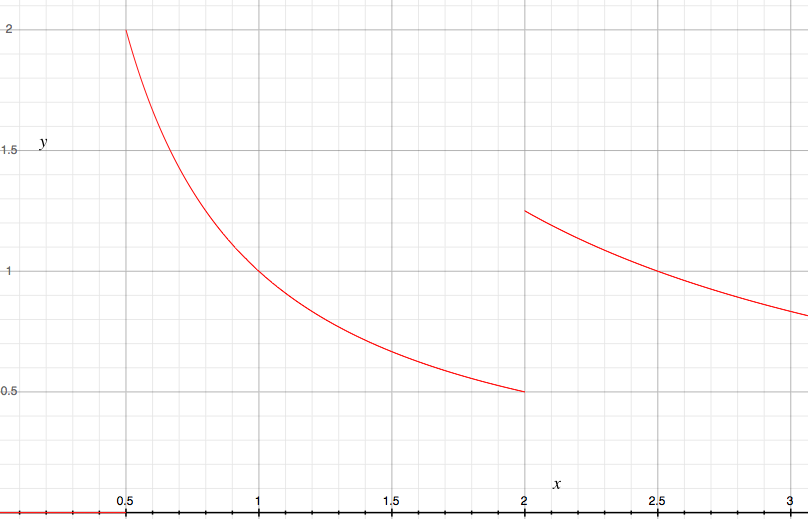
\includegraphics[width=10cm]{p2}
\end{center}
\end{figure}
If the charges are opposite signs, then that will be encompased inside the same equations as above.
The plot will change slightly:
\begin{figure}[H]
\begin{center}
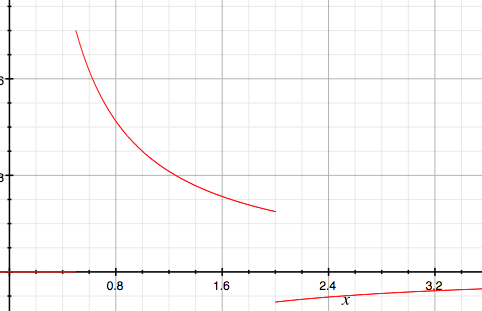
\includegraphics[width=10cm]{p3}
\end{center}
\end{figure}
Depending on which sign is larger this could look different.  The big thing to notice is that the
electric field inside is going to remain the same regardless of the outside charge.  Gauss' law
explains this phenomena with how it defines the integrating surface.

\newpage

3) \textbf{6.11:}
\begin{figure}[H]
\begin{center}
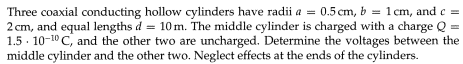
\includegraphics[width=14cm]{f3}
\end{center}
\end{figure}

The electric field inside the middle cylinder is going to be 0, since there is no enclosed charge.
This makes the voltage also 0, since the integral of the electric field over this difference is 0.
The electric field from the middle cylinder to the outer one can be found using a similar method to
that of the last problem.  We find it to be:
\[
  \frac{1.5\cdot 10^{-10}/10}{2\pi \epsilon_0 r}
\]
We can use this to find the voltage:
\[
  V = \int_{0.01}^{0.02} \frac{1.5\cdot 10^{-10}/10}{2\pi \epsilon_0 r} dr = 
  \frac{1.5\cdot 10^{-10}/10}{2\pi \epsilon_0} \ln{\frac{0.02}{0.01}} = 0.1869 V
\]

4) \textbf{6.14:}
\begin{figure}[H]
\begin{center}
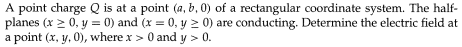
\includegraphics[width=14cm]{f4}
\end{center}
\end{figure}

This point charge is going to feel the effects on each side as if another charge was on the other
side of each plane.  We can sum the fields from each "mirror image" charge to find the field at
any point.
\[
  E(x,y,0) = \frac{kQ}{(x-a)^2+(y-b)^2} + \frac{kQ}{(x+2a)^2+(y-b)^2} + \frac{kQ}{(x-a)^2+(y+2b)^2}
\]


\newpage

5) \textbf{7.7:}
\begin{figure}[H]
\begin{center}
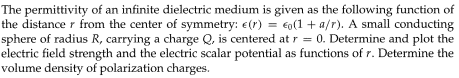
\includegraphics[width=14cm]{f5}
\end{center}
\end{figure}
The electric field strength can be found as a simple functino of $r$:
\[
  E(r) = \frac{Q}{4\pi\epsilon_1 r^2} \Rightarrow \frac{Q}{4\pi\epsilon_0(1+a/r) r^2} \text{ for } r>R \text{ else } E = 0
\]
To find to scalar potential, we can preform the following integral:
\[
  V = \int_{R}^{r} \frac{Q}{4\pi\epsilon_0(a+r)r}dr = \frac{Q}{4\pi\epsilon_0}(\ln(\frac{r}{r+1}) - \ln(\frac{R}{R+1}))
\]
The volume density of polarization charges is the charge $Q$ devided by the total volume of the sphere:
\[
  \frac{Q}{4/3\pi R^3}
\]
\newpage

6) \textbf{8.15:}
\begin{figure}[H]
\begin{center}
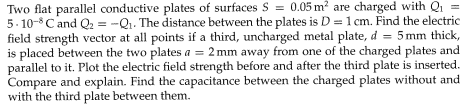
\includegraphics[width=14cm]{f6}
\end{center}
\end{figure}

Without the charged plate in between the other two, we can find the Electric field quite easily:
\[
  E = \frac{\sigma}{\epsilon_0}\text{ where } \sigma = \frac{Q}{A} \Rightarrow E = 113000 N/C
\]
With the new uncharged plate, the electric field remains unchaged.  This is because the perfect
conductor will move a charge $Q$ towards the plate 1 and a charge $-Q$ towards the other plate.
The only difference is that the electric field in that 5mm where the plate is becomes 0.  The plot
would look like so:
\begin{figure}[H]
\begin{center}
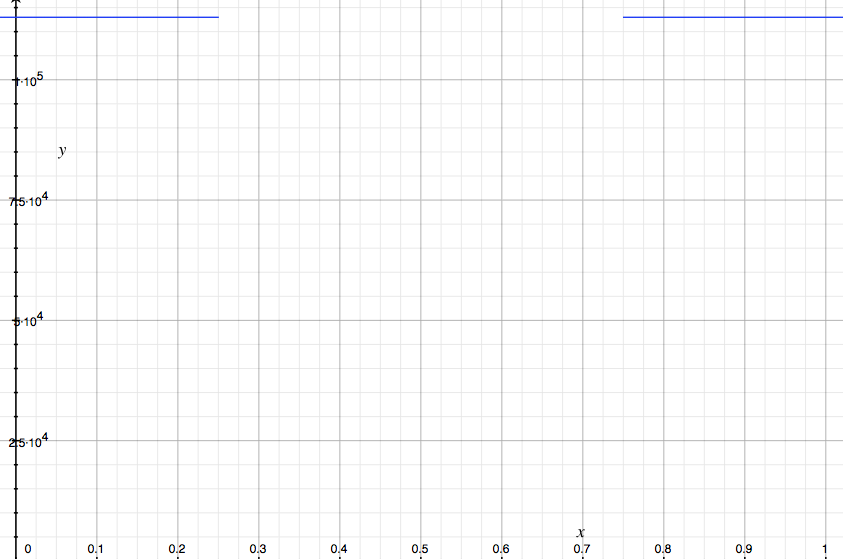
\includegraphics[width=9cm]{p4}
\end{center}
\end{figure}
The capacitance has changed, since the sum of the electric field over the distance is now different.
In the original case, the voltage is:
\[
  V = E \cdot d = 1130 Volts
\]
And in the second case:
\[
  V = E \cdot (0.25cm) + E\cdot (0.25cm) = 565 Volt
\]

\newpage

7) \textbf{8.20:}
\begin{figure}[H]
\begin{center}
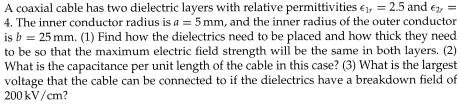
\includegraphics[width=14cm]{f7}
\end{center}
\end{figure}

Gauss' law tells us that the electric field on the surface of the inner dielectric is $\frac{Q'}{2\pi\epsilon_{1r} r}$.
Note that the thinckness and position of this inner dielectric doesnt matter.  The electric field in
the outer dielectric is 0.  The outer and inner electric can never be the same unless there is no
charge running through the cable.  The capacitance per unit length can be found quite easily, first we
find the voltage:
\[
  V = \frac{Q'}{2\pi\epsilon_{1r}}\ln(\frac{b}{a})
\]
\[
  C' = \frac{Q'}{V} = \frac{2\pi\epsilon_{1r}}{\ln\frac{b}{a}} = 9.76 F/m
\]
The largest voltage that can be applied is:
\[
  V = 200kV/cm \cdot 20mm = 400kV
\]

8) \textbf{9.15:}
\begin{figure}[H]
\begin{center}
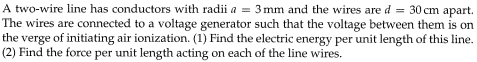
\includegraphics[width=14cm]{f8}
\end{center}
\end{figure}
The field per unit length can be found in the textbook as
\[
  E' = \frac{Q'}{2\pi\epsilon_0(30cm)} \text{ where } Q' = \pi\epsilon_0V/\ln{(30cm/3mm)} = 506569 V/m
\]
The force per unit lenght can also be found by an equation in the book:
\[
  F = -Q'E' = 1.071 N/m
\]


\end{document}
